\documentclass[aspectratio=169]{beamer}
\usepackage[utf8]{inputenc}
\usepackage[ngerman]{babel}
\usetheme{Boadilla}
\setbeamertemplate{navigation symbols}{}

\title{Einf\"uhrung in Quanten-Computing}
\author{M. Brinkmann, K. Ortel, \bf{P. Tesarik}}
\date{\today}

\begin{document}
\maketitle

\section{Abschnitt i}
\begin{frame}
  \frametitle{Klassische Quantenchemie}

  \begin{definition}
    Beschreibung der elektronischen Struktur von Atomen und Molek\"ulen und die Auswirkung auf ihre Reaktionsf\"ahigkeit und Eigenschaften. 
  \end{definition}
  \pause 
  \begin{itemize}
    \item L\"osung der zeit(un)abh\"angigen Schr\"odinger Gleichung: $ \hat{\mathcal{H}} \Psi = \mathcal{E} \Psi $
%    \pause
    \item Genauigkeit abh\"angig von den Ans\"atzen von $ \Psi $ und weiteren N\"aherungen
%    \pause
    \item Komplexit\"at der Rechnung abh\"angig von Zahl der Elektronen und Basissatz
%    \pause
    \item L\"osungsverfahren: Iterativ und mit hohen Rechenzeitkosten 
  \end{itemize}

\end{frame}

%\begin{frame}
%  \frametitle{Klassische Quantenchemie}
%\end{frame}

\section{Abschnitt ii}
\begin{frame}
  \frametitle{Quantenchemie mit Quantensimulation}
  \begin{definition}[der Idee]
  Der Quantenprozessor \"ubernimmt die f\"ur klassische Systeme schwierigen Rechnungen
  \end{definition}

  \begin{itemize}
  \item Quantenphasen N\"aherungsalgorithmus
  \item Variabler Quanten-Eigenl\"oser
  \end{itemize}
\end{frame} 

\begin{frame}
  \frametitle{Variabler Quanten-Eigenl\"oser}
  \begin{enumerate}
  \item Parameter nach Energie erstellen und Modell generieren (klassisch)
  \item Testzust\"ande des Systems berechnen (quantum)
  \item Energien auslesen (quantum)
  \item Energien auswerten (klassisch)
  \item Gehe zu 1
  \end{enumerate}
\end{frame}

\begin{frame}
  \frametitle{Variabler Quanten-Eigenl\"oser}
  \begin{figure}
  \centering
  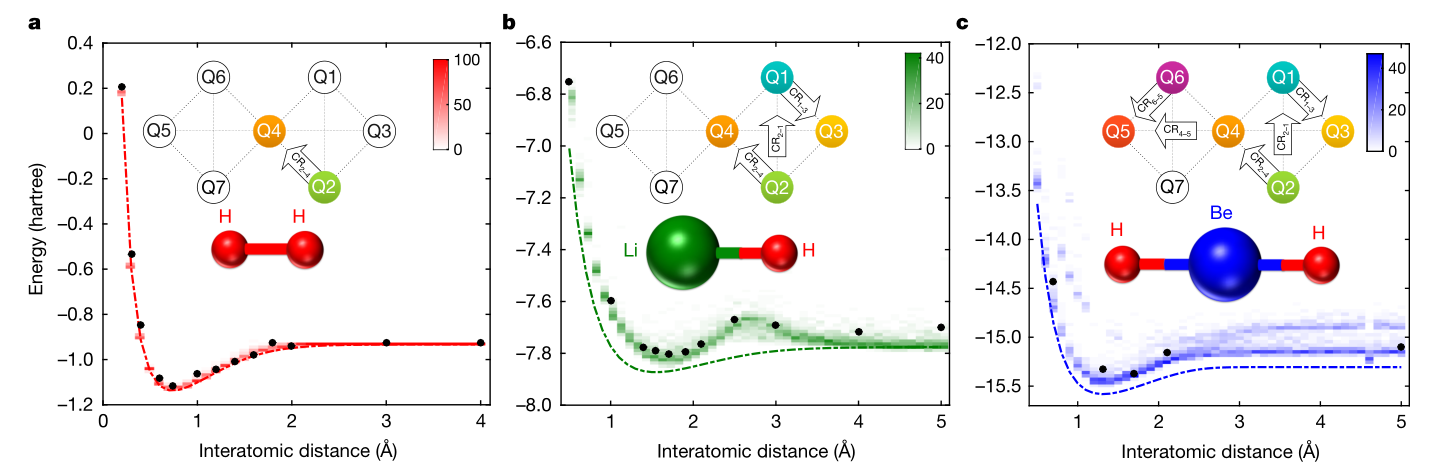
\includegraphics[width=\textwidth]{pes}
  \caption{Kandala et. al., https://arxiv.org/abs/1704.05018}
  \end{figure}
\end{frame}

\end{document}
